\section{Програмна реалізація системи}
\subsection{Особливості програмної реалізації системи, що розробляється}
Для розробки програмної системи була використані мова програмування Kotlin та застосовані патерни проектування типу GoF.

Були застосовані принципи SOLID~\cite{Arch2007}:
\begin{enumerate}
	\item Принцип єдиного обов'язку --- принцип об'єктно-орієнтованого програмування, який означає, що клас має бути створений для виконання лише однієї задачі, яку він повинен повністю інкапсулювати.
	      Отже, всі сервіси цього класу мають бути повністю підпорядковані її виконанню.
	      Результатом слідування цій концепції є наявність лише однієї причини для зміни класу.
	\item Принцип відкритості/закритості --- принцип об'єктно-орієнтованого програмування, який означає, що програмні сутності, такі як класи, модулі, функції, методи та ін. мають бути <<відкритими для розширення та закритими для змін>>.
	      Це означає, що вони можуть надавати можливість змінювати свою поведінку без або з мінімальними змінами коду.
	\item Принцип заміщення Лісков --- якщо $S$ підтип $T$, тоді об'єкти типу $T$ в програмі можуть бути заміщені об'єктами типу $S$ без будь-яких змін бажаних властивостей цієї програми.
	\item Принцип розділення інтерфейсів --- принцип схожий із принципом єдиного обов'язку.
	      Застосування даного принципу полягає у розділі занадто <<товстих>> інтерфейсів на менші та специфічні, щоб їх клієнти знали лише про ті методи, що необхідні для них у роботі.
	      Як результат, при зміні певного функціоналу, незмінними мають лишитися ті класи, що не використовують його.
	      Тобто виконання цього принципу допомагає системі залишатися гнучкою при внесенні до неї змін та лишатися простою для рефакторингу.
	\item Принцип інверсії залежностей.
	      Принцип формулюється наступним чином: модулі вищого рівня не повинні залежати від модулів нижчого рівня, обидва типи модулів повинні залежати від абстракцій; абстракції не повинні залежати від деталей реалізації, деталі реалізації повинні залежати від абстракцій.
\end{enumerate}

Система реалізована у парадігмі чистої архітектури, яка полягає в розділенні системи на 3 рівні~\cite{Arch2007}:
\begin{enumerate}
	\item Рівень даних --- рівень даних у чистому вигляді, що складається з сутностей, які є основними бізнес-правилами системи.
	\item Доменний рівень --- рівень бізнес-логіки додатку, що відповідає за основний функціонал системи, її поведінку та правила, що стосуються конкретного додатку.
	\item Рівень представлення --- рівень користувацького інтерфейсу, відображення даних, обробки користувацьких подій.
\end{enumerate}

\subsection{Тестування програмного забезпечення}
\subsubsection{Загальна теорія тестування}
Тестування --- перевірка відповідності реальної поведінки програми очікуваній, що здійснюється на кінцевому наборі тестів, який був обраний певним чином.
У більш широкому сенсі, тестування --- це одна з технік контролю якості, що включає в себе активності з планування робіт, проектування тестів, виконання тестування і аналізу отриманих результатів~\cite{Swebok}.

Верифікація --- це процес оцінки системи або її компонентів з метою визначення чи задовольняють результати поточного етапу розробки умовам, що були сформовані на початку цього етапу.
Тобто чи виконуються наші цілі, терміни, завдання по розробці проекту, визначені на початку поточної фази~\cite{Swebok}.

Валідація --- це визначення відповідності ПО, що розроблюється очікуванням і потребам користувача, вимогам до системи~\cite{Swebok}.

\subsubsection{Тестування програмної системи}
На першому етапі тестування необхідно провести модульне тестування усіх компонентів системи, які можуть бути протестовані окремо від інших у штучному середовищі тестування.
Для Unit-тестування використовується засоб автоматизації тестування Kotest.

Такий вибір зумовлений простотою інтеграції з Kotlin.
Kotest надає великий об'єм валідаційних методів, завдяки яким можна легко та ефективно тестувати як модулі обробки даних та взаємодії з базами даних, так і модулі вводу та виводу інформації~\cite{Kotest}.

Фрагмент застосованих Kotest тестів для валідації коректної роботи класу \texttt{GlobeHipster} приведено нижче:
\lstinputlisting{code/tests.kt}

\subsection{Інтерфейс програмного забезпечення}
Розроблена програмна система має консольний інтерфейс. Для запуску моделювання необхідно виконати такі команди:
\begin{lstlisting}
> jar kagent.jar --period=14 --time=5 configuration_a.json configuration_b.json
\end{lstlisting}
\begin{description}
	\item[де] \texttt{kagent.jar} --- назва бінарного файла програмної системи;
	\item \texttt{--period=14} --- період поповнення запасів регіональними та національними складами, у днях;
	\item \texttt{--time=5} --- час моделювання системи, у секундах;
	\item \texttt{configuration\_a.json} --- шлях до файлу конфігурації першого варіанта логістичної системи;
	\item \texttt{configuration\_b.json} --- шлях до файлу конфігурації другого варіанта логістичної системи.
\end{description}

В процесі моделювання логістичної системи у консоль виводиться поточний стан логістичної системи.
Фрагмент логування початкової загрузки конфігурації логістичної системи:
\begin{lstlisting}
Connecting Киев to Пирятин by 154.0 km. road
Connecting Житомир to Винница by 127.0 km. road
Connecting Николаев to Мелитополь by 299.0 km. road
Connecting Николаев to Саки by 325.0 km. road
Connecting Днепропетровск to Днепродзержинск by 45.0 km. road
Connecting Львов to Дубляны by 9.0 km. road
\end{lstlisting}

Фрагмент логування процесу моделювання логістичної системи:
\begin{lstlisting}
[432]
.     Current time is 432 days.
.    service level is 87%.
. avg. stock level is 92%.
[433]
.     Current time is 433 days.
.    service level is 88%.
. avg. stock level is 92%.
[434]
.     Current time is 434 days.
.    service level is 88%.
. avg. stock level is 91%.
\end{lstlisting}

Для генерації дампу поточного стану системи у файл необхідно натиснути клавішу <<S>> під час процесу моделювання, для призупинення виконування програми необхідно натиснути клавішу <<P>>.
Графічний інтерфейс складається з двох частин: меню та панелі поточного стану моделі.

Після закінчення часу на моделювання системи показується окно з динамікою зміни рівня сервісу за час моделювання (рисунок~\ref{fig:graph_sample}).

\begin{figure}[H]
	\centering
	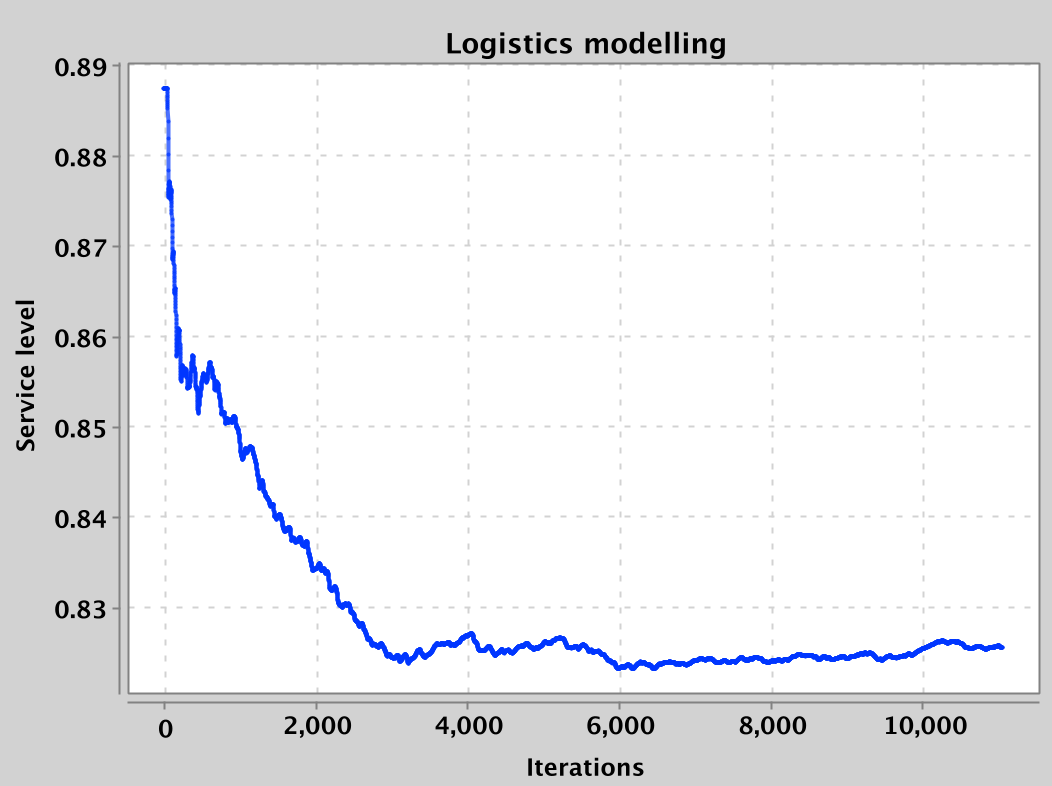
\includegraphics[width=0.6\textwidth]{graph_sample}
	\caption{Динаміка зміни рівня сервісу}
	\label{fig:graph_sample}
\end{figure}

\subsection{Аналіз продуктивності програмного забезпечення}
Розроблений програмний продукт широко використовує паралельні обчислення. 
В якості основи для паралельних обчислень було використано технологію Kotlin coroutines.

Для порівняння роботи програми у багатопотоковому режимі та однопотоковому режимі був проведений експеримент: моделювання логістичної системи~\cite{Годлевський2019} з обмеженої кількістю агентів на регіональному шару. Результат експерименту представлено на рисунку~\ref{fig:performance}.

\begin{figure}[H]
	\centering
	\begin{tikzpicture}
		\begin{axis}[
				scaled y ticks = false,
				xlabel={Кількість кінцевих споживачів продукції},
				xlabel near ticks,
				ylabel={Ітерацій за 100 мілісекунд},
				ylabel near ticks,
				ymajorgrids=true,
				line width=0.4mm,
				grid style=dashed,
			]
			\addplot table [x=n, y=i] {data/test_cpu.csv};
			\addplot table [x=n, y=z] {data/test_cpu.csv};
			\legend{багатопотоковий режим,однопотоковий режим}
		\end{axis}
	\end{tikzpicture}
	\caption{Результати оцінки продуктивності~\acrshort{sw}}
	\label{fig:performance}
\end{figure}

Програмний продукт у багатопотоковому режимі працює в $\~5$ разів швидше ніж у однопотоковому режимі. 
Це обумовлено тим що експеримент проводився на комп'ютері з чотирма ядрами процессору і у многопоточному режимі програма використовує всі ресурси всіх процесорів, а в однопотоковому режимі тільки один.  

\subsection{Аналіз результатів дослідження}
Початкова конфігурація була взята з роботи~\cite{Годлевський2019} яка в свою чергу базується на роботі <<Моделі і інформаційна технологія стратегічного управління логістичною системою дистрибуції>>~\cite{Stankevich}.

З метою формування множини ефективних рішень конфігурації логістичної системи в роботі були приведені прорахунки для двох варіантів базового рівня сервісу на регіональних складах: $84.13\%$, $97.72\%$. Для кожного базового рівня сервісу розглядалися тривалості циклів замовлень з виробничого на національний і далі на регіональний рівні: 2, 3 і 4 тижні.

Таким чином було сформовано 36 конфігурацій логістичних мереж, для кожної з котрих було проведено моделювання рівня сервісу.

Результати експерименту приведені в таблиці~\ref{tab:results}.

{
\small
\tabulinesep=1.2mm
\begin{longtabu} to \textwidth {|X[1,c]|X[1,c]|X[1,c]|X[1,c]|X[1,c]|}
	\caption{Результати експерименту моделювання конфігурацій логістичних систем}
	\label{tab:results} \\
	\hline
	Кількість регіональних складів & Тривалість циклу, тижнів & Базовий рівень страхового запасу, \% & Сумарні логістичні витрати~\cite{Годлевський2019} & Мережевий рівень сервісу \\
	\hline
	\endfirsthead
	\caption*{Закінчення таблиці \thetable{}}\\
	\hline
	Кількість регіональних складів & Тривалість циклу, тижнів & Базовий рівень страхового запасу, \% & Сумарні логістичні витрати~\cite{Годлевський2019} & Мережевий рівень сервісу \\
	\hline
	\endhead
	5 & \multirow{4}{*}{2} & \multirow{12}{*}{$84.13$} & $183729.3882$ & $0.864868$ \\ \cline{1-1}\cline{4-5}
	6 & & & $185253.5535$ & $0.868993$ \\ \cline{1-1}\cline{4-5}
	7 & & & $185649.9391$ & $0.871659$ \\ \cline{1-1}\cline{4-5}
	8 & & & $185935.0956$ & $0.873573$ \\ \cline{1-2}\cline{4-5}

	5 & \multirow{4}{*}{3} & & $195332.5978$ & $0.830533$ \\ \cline{1-1}\cline{4-5}
	6 & & & $196856.7631$ & $0.831683$ \\ \cline{1-1}\cline{4-5}
	7 & & & $197253.1487$ & $0.831786$ \\ \cline{1-1}\cline{4-5}
	8 & & & $197538.3052$ & $97$ \\ \cline{1-2}\cline{4-5}

	5 & \multirow{4}{*}{4} & & $206935.8074$ & $0.793313$ \\ \cline{1-1}\cline{4-5}
	6 & & & $208459.9727$ & $0.800558$ \\ \cline{1-1}\cline{4-5}
	7 & & & $208856.3583$ & $0.804958$ \\ \cline{1-1}\cline{4-5}
	8 & & & $209141.5148$ & $0.808666$ \\ \hline

	5 & \multirow{4}{*}{2} & \multirow{12}{*}{$97.72$} & $187478.0538$ & $0.931035$ \\ \cline{1-1}\cline{4-5}
	6 & & & $189002.2191$ & $0.938148$ \\ \cline{1-1}\cline{4-5}
	7 & & & $189398.6047$ & $0.939289$ \\ \cline{1-1}\cline{4-5}
	8 & & & $189683.7612$ & $0.940954$ \\ \cline{1-2}\cline{4-5}

	5 & \multirow{4}{*}{3} & & $200955.5962$ & $0.895327$ \\ \cline{1-1}\cline{4-5}
	6 & & & $202479.7615$ & $0.896253$ \\ \cline{1-1}\cline{4-5}
	7 & & & $202876.1471$ & $0.898870$ \\ \cline{1-1}\cline{4-5}
	8 & & & $203161.3036$ & $0.900588$ \\ \cline{1-2}\cline{4-5}

	5 & \multirow{4}{*}{4} & & $214433.1386$ & $0.859070$ \\ \cline{1-1}\cline{4-5}
	6 & & & $215957.3039$ & $0.867487$ \\ \cline{1-1}\cline{4-5}
	7 & & & $216353.6895$ & $0.870390$ \\ \cline{1-1}\cline{4-5}
	8 & & & $216638.846$ & $0.877827$ \\ \hline
\end{longtabu}
}

Візуалізація зміни рівня сервісу представлені на рисунках~\ref{fig:graph_84},~\ref{fig:graph_99}.

\begin{figure}[H]
	% \def\axisdefaultwidth{14cm}
	% \def\axisdefaultheight{10сm}
	\centering
	\begin{tikzpicture}
		\begin{axis}[
				legend style={font=\footnotesize,at={(1.6,1.0)},anchor=north east},
				xmin=0,
				xmax=10000,
				xlabel={Номер ітерації моделювання},
				xlabel style={yshift=-1cm},
				ylabel={Рівень сервісу},
				ylabel near ticks,
				ymajorgrids=true,
				grid style=dashed,
				line width=0.4mm,
				mark size=0pt,
				mark = none,
				smooth
			]
			\addplot table [x=i, y=1] {data/dynamic_84.csv};
			\addplot table [x=i, y=2] {data/dynamic_84.csv};
			\addplot table [x=i, y=3] {data/dynamic_84.csv};
			\addplot table [x=i, y=4] {data/dynamic_84.csv};
			\addplot table [x=i, y=5] {data/dynamic_84.csv};
			\addplot table [x=i, y=6] {data/dynamic_84.csv};
			\addplot table [x=i, y=7] {data/dynamic_84.csv};
			\addplot table [x=i, y=8] {data/dynamic_84.csv};
			\addplot table [x=i, y=9] {data/dynamic_84.csv};
			\addplot table [x=i, y=10] {data/dynamic_84.csv};
			\addplot table [x=i, y=11] {data/dynamic_84.csv};
			\addplot table [x=i, y=12] {data/dynamic_84.csv};
			\legend{5 складів; 2 тижня,6 складів; 2 тижня,7 складів; 2 тижня,8 складів; 2 тижня,5 складів; 3 тижня,6 складів; 3 тижня,7 складів; 3 тижня,8 складів; 3 тижня,5 складів; 4 тижня,6 складів; 4 тижня,7 складів; 4 тижня,8 складів; 4 тижня}
		\end{axis}
	\end{tikzpicture}
	% 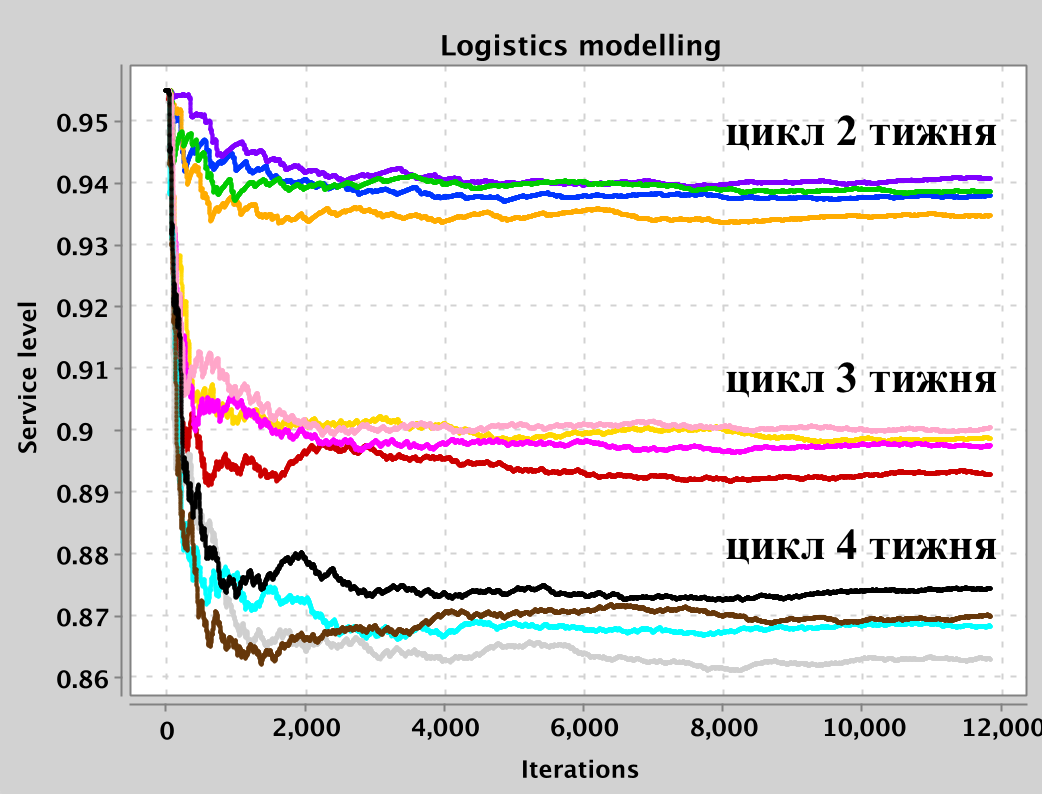
\includegraphics[width=0.6\textwidth]{graph_99}
	\caption{Динаміка зміни рівня сервісу для групи конфігурацій з базовим рівнем страхового запасу рівним $84.13$}
	\label{fig:graph_84}
\end{figure}

\begin{figure}[H]
	% \def\axisdefaultwidth{14cm}
	% \def\axisdefaultheight{10сm}
	\centering
	\begin{tikzpicture}
		\begin{axis}[
				legend style={font=\footnotesize,at={(1.6,1.0)},anchor=north east},
				xmin=0,
				xmax=10000,
				xlabel={Номер ітерації моделювання},
				xlabel style={yshift=-1cm},
				ylabel={Рівень сервісу},
				ylabel near ticks,
				ymajorgrids=true,
				grid style=dashed,
				line width=0.4mm,
				mark size=0pt,
				mark = none,
				smooth
			]
			\addplot table [x=i, y=1] {data/dynamic_97.csv};
			\addplot table [x=i, y=2] {data/dynamic_97.csv};
			\addplot table [x=i, y=3] {data/dynamic_97.csv};
			\addplot table [x=i, y=4] {data/dynamic_97.csv};
			\addplot table [x=i, y=5] {data/dynamic_97.csv};
			\addplot table [x=i, y=6] {data/dynamic_97.csv};
			\addplot table [x=i, y=7] {data/dynamic_97.csv};
			\addplot table [x=i, y=8] {data/dynamic_97.csv};
			\addplot table [x=i, y=9] {data/dynamic_97.csv};
			\addplot table [x=i, y=10] {data/dynamic_97.csv};
			\addplot table [x=i, y=11] {data/dynamic_97.csv};
			\addplot table [x=i, y=12] {data/dynamic_97.csv};
			\legend{5 складів; 2 тижня,6 складів; 2 тижня,7 складів; 2 тижня,8 складів; 2 тижня,5 складів; 3 тижня,6 складів; 3 тижня,7 складів; 3 тижня,8 складів; 3 тижня,5 складів; 4 тижня,6 складів; 4 тижня,7 складів; 4 тижня,8 складів; 4 тижня}
		\end{axis}
	\end{tikzpicture}
	% 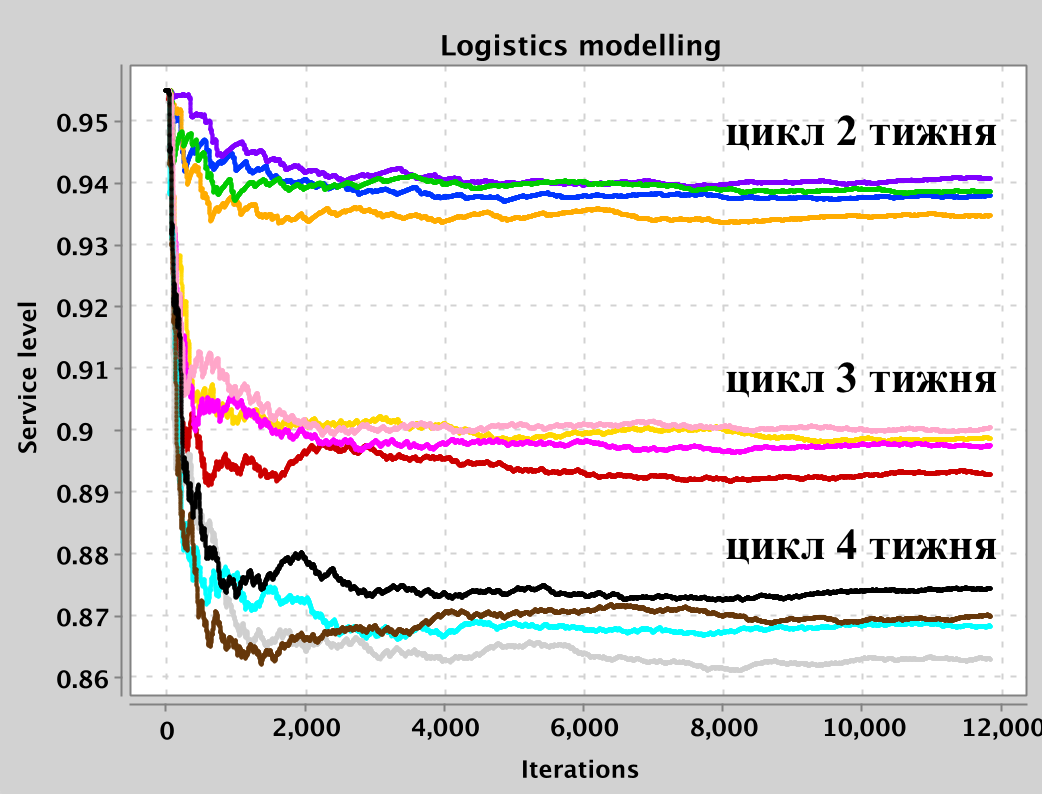
\includegraphics[width=0.6\textwidth]{graph_99}
	\caption{Динаміка зміни рівня сервісу для групи конфігурацій з базовим рівнем страхового запасу рівним $97.72$}
	\label{fig:graph_99}
\end{figure}

Наглядна графічна інтерпретація результатів з таблиці~\ref{tab:results} зображена на рисунку~\ref{fig:results}.

\begin{figure}[H]
	\centering
	\begin{tikzpicture}
		\begin{axis}[
				scaled y ticks = false,
				xlabel={Сумарні логістичні витрати},
				xlabel style={yshift=-1cm},
				ylabel={Мережевий рівень сервісу},
				ylabel near ticks,
				enlargelimits=false,
				line width=0.4mm,
				ymajorgrids=true,
				grid style=dashed,
			]
			\addplot+[
				only marks,
				scatter,
				mark=halfcircle*,
				mark size=2.9pt]
			table[meta=y]
				{data/results.csv};
		\end{axis}
	\end{tikzpicture}
	\caption{Результати експерименту моделювання конфігурацій логістичних систем}
	\label{fig:results}
\end{figure}

Проведемо аналіз отриманих результатів.
Незалежно від тривалості циклів замовлень рівень сервісу збільшується зі збільшенням кількості регіональних складів.
Це можна пояснити тим, що збільшується загальний розмір страхових запасів.
Мережевий рівень сервісу зменшується зі збільшенням тривалості циклів замовлень. Це пов'язано з тим, що при меншому циклі замовлень є більше можливостей на адаптацію до змін попиту.
Зі збільшенням базового рівня сервісу збільшується рівень мережевого сервісу.
Виходячи з проведеного аналізу, можна зробити висновок, що безліч ефективних рішень знаходиться в лівому верхньому кутку графіка (рис.~\ref{fig:results}). Залежно від пріоритету експерту по відношенню до критеріїв: сумарні логістичні витрати, мережевий рівень сервісу вибирається прийнятна конфігурація логістичної системи.

Подальше використання отриманих результатів пов'язане з визначенням стійкості рівня сервісу до різноманітних надзвичайних ситуацій. Отримані результати є основою для формування організаційної структури управління логістичною системою дистрибуції.
